\section*{H/4/9. feladat: Nyomás meghatározás csővezetékrendszerben}
\addcontentsline{toc}{section}{H/4/9. feladat: Nyomás meghatározás csővezetékrendszerben}

\begin{tabular}{ | p{2cm} | p{14cm} | } 
	\hline
	Név & Vasáros Mátyás \\ 
	\hline
	Szak & Mechatronikai mérnök\\ 
	\hline
	Félév & 2019/2020 II. (tavaszi) félév \\ 
	\hline
\end{tabular}
\vspace{0.5cm}

\noindent Egy az ábrán látható csővezetékrendszer 1-es pontjában kell meghatározni a statikus nyomást, ha a következő adatokat ismerjük. A csövek átmérője $d = \SI{50}{\mm}$, az ábrán feltüntetett csőhosszak $l_{1} = \SI{2}{\m}$, $l_{2} = \SI{0,1}{\m}$, $l_{3} = \SI{0,1}{\m}$ és $l_{4} = \SI{30}{\m}$, a szelep ellenállási tényezője $\zeta_{T} ={0,8}$, a könyökök ellenállási tényezője $\zeta_{k} = {0,15}$, a térfogatáram $\dot{V}=\SI{180}{\liter\per\minute}$, a csősúrlódási tényező $\lambda={0,025}$, a folyadék(víz) sűrűsége $\rho=\SI{e3}{\kilogram\per\meter\cubed}$, a külső légnyomás $p_{0}=\SI{e5}{\pascal}$.


\begin{figure}[h]
	\centering
	\label{figure:sm}
	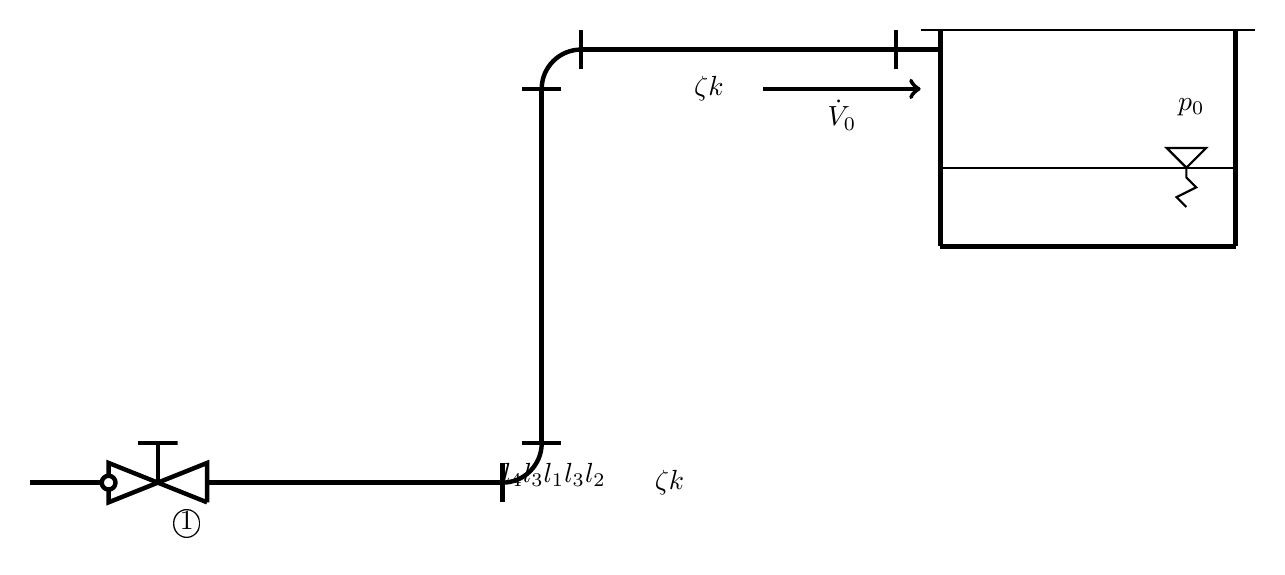
\begin{tikzpicture}
		
	% Változók
	
	\pgfmathsetmacro{\zoom}{2.5}		   	%scaleli a rajzot
	\pgfmathsetmacro{\Legy}{2*\zoom}	 %L1 hosszméret
	\pgfmathsetmacro{\Lketto}{2*\zoom}	 %L2 hosszméret
	\pgfmathsetmacro{\Lharom}{0.2*\zoom} %L3 hosszméret
	\pgfmathsetmacro{\Lnegy}{1.5*\zoom}	 %L4 hosszméret
	\pgfmathsetmacro{\Thossz}{1.5*\zoom}	 %Tartály hossza
	\pgfmathsetmacro{\Tmag}{1*\zoom}		 %Tartály magassága
	\pgfmathsetmacro{\Csat}{0.1*\zoom}	 %Csatlakozóperem, tartályperem, kukacvonal méret
	\pgfmathsetmacro{\Kukac}{0.05*\zoom}
	
	\pgfmathsetmacro{\Tnullx}{\Lharom+\Lketto+0.025*\zoom}
	\pgfmathsetmacro{\Tnully}{\Legy+\Lharom}
	\pgfmathsetmacro{\Vizsz}{1}	%vízszint
	\pgfmathsetmacro{\Trix}{1.25*\zoom}	%kis háromszög helye a vízfelszínen
	\pgfmathsetmacro{\Vszel}{0.5*\zoom} %szelep hossza
	\pgfmathsetmacro{\Vmag}{0.1*\zoom} %szelep magassága
	\pgfmathsetmacro{\Vkor}{0.035*\zoom} %szelepbogyóméret
	\pgfmathsetmacro{\Vekt}{0.4*\zoom}
	
	% Csövek idomok és csőperemek (0,0 az alsó könyök bal oldalánál)
	\draw[ultra thick] 	(-\Lnegy,0)--(0,0); 																	%l4 vonal
	\draw[ultra thick] (0,-\Csat)--(0,\Csat);																	%első könyök előtti perem
	\draw[ultra thick] (0, 0) arc [radius=\Lharom, start angle=270, end angle=360];								%első könyök
	\draw[ultra thick] 	(\Lharom-\Csat,\Lharom)--(\Lharom+\Csat,\Lharom);										%első könyök utáni perem
	\draw[ultra thick] 	(\Lharom,\Lharom)--(\Lharom,\Legy);														%l1 vonal
	\draw[ultra thick] 	(\Lharom-\Csat,\Legy)--(\Lharom+\Csat,\Legy);											%második könyök előtti perem
	\draw[ultra thick] (\Lharom,\Legy) arc [radius=\Lharom, start angle=180, end angle=90];						%második könyök
	\draw[ultra thick] (2*\Lharom, \Legy+\Lharom+\Csat)--(2*\Lharom,\Legy+\Lharom-\Csat);						%második könyök utáni perem
	\draw[ultra thick] (2*\Lharom, \Legy+\Lharom)--(\Lketto,\Legy+\Lharom);										%l2 vonal
	\draw[ultra thick] (\Lketto,\Lharom+\Legy-\Csat)--(\Lketto,\Lharom+\Legy+\Csat); 							%tartály előtti perem
	\draw[ultra thick] (\Lketto,\Legy+\Lharom)--(\Tnullx,\Tnully);												%tartály betöltő csonk
	
	% Tartály
	\draw[ultra thick] (\Tnullx,\Tnully+\Csat)--(\Tnullx,\Tnully-\Tmag);										%tartály ball oldal
	\draw[ultra thick] (\Tnullx,\Tnully-\Tmag)--(\Tnullx+\Thossz,\Tnully-\Tmag);								%tartály alja
	\draw[ultra thick] (\Tnullx+\Thossz,\Tnully-\Tmag)--(\Tnullx+\Thossz,\Tnully+\Csat);						%tartály jobb oldala		
	\draw[thick] (\Tnullx-\Csat,\Tnully+\Csat)--(\Tnullx+\Thossz+\Csat,\Tnully+\Csat);							%tartály fedele
	\draw[thick] (\Tnullx,\Tnully-\Tmag+\Vizsz)--(\Tnullx+\Thossz,\Tnully-\Tmag+\Vizsz);						%vízfelszín
	\draw[thick] (\Tnullx+\Trix,\Tnully-\Tmag+\Vizsz) -- 
		(\Tnullx+\Trix-\Csat,\Tnully-\Tmag+\Vizsz+\Csat)--		
		(\Tnullx+\Trix+\Csat,\Tnully-\Tmag+\Vizsz+\Csat)--
		(\Tnullx+\Trix,\Tnully-\Tmag+\Vizsz);						%kis háromszög	
	
	\draw[thick](\Tnullx+\Trix,\Tnully-\Tmag+\Vizsz)--
		(\Tnullx+\Trix,\Tnully-\Tmag+\Vizsz-\Kukac)--
		(\Tnullx+\Trix+\Kukac,\Tnully-\Tmag+\Vizsz-2*\Kukac)--
		(\Tnullx+\Trix-\Kukac,\Tnully-\Tmag+\Vizsz-3*\Kukac)--
		(\Tnullx+\Trix,\Tnully-\Tmag+\Vizsz-4*\Kukac);		%kukacvonal
	
	% Csap
	\draw[ultra thick] (-\Lnegy,-\Vmag)--
		(-\Lnegy,\Vmag)--
		(-\Lnegy-\Vszel,-\Vmag)--
		(-\Lnegy-\Vszel,0-\Vkor);	
			
	\draw[ultra thick] (-\Lnegy-\Vszel,0) circle (\Vkor);
	\draw[ultra thick] (-\Lnegy-\Vszel,0+\Vkor)--
		(-\Lnegy-\Vszel,\Vmag)--
		(-\Lnegy,-\Vmag);	%test
		
	\draw[ultra thick] (-\Lnegy-\Vszel/2,0)--
		(-\Lnegy-\Vszel/2,2*\Vmag)--
		(-\Lnegy-\Vszel/2+\Csat,2*\Vmag)--
		(-\Lnegy-\Vszel/2-\Csat,2*\Vmag);	%szelep
		
	\draw[ultra thick] (-\Lnegy-\Vszel-\Vkor,0)--(-\Lnegy-\Vszel-1,0);	%bejövő ág
	
	%Méretek
	\pgflength[ xa={-\Lnegy}, ya={-0}, xb={0}, yb={0},ra={0.65} ]{$l_{4}$};				%l4			
	\pgflength[ xa={\Lharom}, ya={0}, xb={\Lharom}, yb={\Lharom},ra={-\Lharom} ]{$l_{3}$};		%l3 alsó	
	\pgflength[ xa={\Lharom}, ya={\Lharom}, xb={\Lharom}, yb={\Legy},ra={-\Lharom} ]{$l_{1}$};		%l1
	\pgflength[ xa={2*\Lharom}, ya={\Legy}, xb={2*\Lharom}, yb={\Lharom+\Legy},ra={-2*\Lharom} ]{$l_{3}$}	%l3 felső	
	\pgflength[ xa={2*\Lharom}, ya={\Lharom+\Legy}, xb={\Lketto}, yb={\Lharom+\Legy},ra={-0.65} ]{$l_{2}$};		%l2	
	
	%Felíratok
	\node[anchor=west] at (\Lharom, 0) {$\zeta{k}$};	 %also kszi
	\node[anchor=west] at (2*\Lharom, \Legy) {$\zeta{k}$};	 %felső kszi
	\node[anchor=north] at (\Tnullx+\Thossz/2, \Legy) {$p_{0}$};	 %p0	
	\node[anchor=north east] at (-\Lnegy-\Vszel,-\Vmag) {\textcircled{1}};	 %1
	\draw[->, ultra thick] (\Lharom-\Vekt+\Lketto/2,\Legy) -- (\Lharom+\Vekt+\Lketto/2,\Legy)
	node[midway, anchor=north,]{$\dot{V}_0$};	%térfogatáram iránya
	
	\end{tikzpicture}
	\caption{Vezetékrendszer}
\end{figure}

\noindent A feladat megoldásához először fel kell venni egy áramvonalat amire fel tudjuk írni a veszteséges Bernoulli egyenletet. Mivel az 1-es pont nyomását keressük, célszerűen az lesz az áramvonal egyik végpontja, a másik végpont a tartály betöltő csonkjánál lesz, ahol ismerjük a nyomást.

\begin{equation}
\dfrac{v_{1}^{2}}{2} + \dfrac{p_{1}}{\varrho} +  gz_{1}
=
\dfrac{v_{2}^{2}}{2} + \dfrac{p_{2}}{\varrho} +  gz_{2} + Y_{vesz}
\end{equation}

\noindent Végezzük el a megfelelő egyszerűsítéseket. Az áramlási sebességet tartalmazó tagok egyenlőek, így kiesnek. Az egyes pont magasságát vegyük $z_{1} = \SI{0}{\m}$-nek. 

\begin{equation}
 \dfrac{p_{1}}{\varrho}
=
 \dfrac{p_{2}}{\varrho} +  gz_{2} + Y_{vesz}
\end{equation}

\noindent A $\varrho$ sűrűséggel átszorozva az egyenletet $p_{1}$ nyomásra rendeztük. Ezzel együtt bontsuk fel a $z_{2}$ értékét.

\begin{equation}
{p_{1}} = {p_{2}} + g (l_{1}+2 \cdot l_{3}) {\varrho} + Y_{vesz} {\varrho}
\end{equation}

\noindent A következő lépés az $Y_{vesz}$ veszteségi tag kifejezése.

\begin{equation}
Y_{vesz} = \zeta \dfrac {v_{atl}^2}{2} =\lambda \dfrac{l_{egyen}}{d} \dfrac {v_{atl}^2}{2}
\end{equation}

\noindent Látható, hogy két ismeretlen tagunk is van, az egyik az $l_{egyen}$ egyenértékű csőhossz a másik pedig a $v_{atl}$ áramlási sebesség, ezeket kell kifejeznünk.

\begin{equation}
l_{egyen} = l_{1}+l_{2}+2l_{3}+l_{4}+\dfrac{d}{\lambda}(\zeta_{T}+2\zeta_{k}+1)
\end{equation}

\begin{equation}
l_{egyen} = \SI{2}{\m}+\SI{2}{\m}+2 \cdot \SI{0,1}{\m}+\SI{30}{\m}+\dfrac{\SI{0,05}{\meter}}{0,025}(0,8+2\cdot 0,15 +1)=\SI{38,4}{\meter}
\end{equation}

\begin{equation}
\dot{V} = v \cdot A 
v=\dfrac{\dot{V}}{A} =\dfrac{\dot{V}}{\dfrac{d^2\pi}{4}} =
	\dfrac{4\dot{V}}{d^2\pi}=
	\dfrac{4\cdot 3 \cdot 10^{-3} \si{\meter\cubed\per\second}}{0,05^2\si{\m\squared}\pi}=
	\dfrac{12\cdot 10^{-3} \si{\meter\cubed\per\second}}{2,5\cdot 10^{-3}\si{\m\squared}\pi}=
	\SI{1,53}{\meter\per\second}
\end{equation}

\noindent A kiszámított értékeket helyettesítsük vissza a $Y_{vesz}$ egyenletébe.

\begin{equation}
Y_{vesz} =\lambda \dfrac{l_{egyen}}{d} \dfrac {v_{atl}^2}{2} =
 0,025 \dfrac{\SI{38,4}{\meter}}{\SI{0,05}{\meter}} \dfrac {1,53^2\si{\meter\squared\per\second\squared}}{2}=
 \SI {22,47}{\joule\per\kilogram}
\end{equation}

\noindent A veszteségi tényezőt az egyszerűsített Bernoulli egyenletbe behelyettesítve meghatározható az egyes pontban a nyomás.

\begin{equation}
{p_{1}} = {p_{2}} + g (l_{1}+2 \cdot l_{3}) {\varrho} + Y_{vesz} {\varrho} = {10^5}\si{\pascal} + \SI {9,81}{\meter\per\second\squared} (\SI{2}{\m} + 2 \cdot \SI{0,1}{\m}) 10^3 \si{\kg\per\meter\cubed} + \SI {22,47}{\joule\per\kilogram} 10^3 \si{\kg\per\meter\cubed}
\end{equation}

\noindent A végeredmény :
\begin{equation}
{p_{1}} = {144052}\si{\pascal}
\end{equation}